\chapter{Case~Study: Fourth~Year~Project~System}

\todo{Fill this in}

\sectionnote {BM}
\section {Overview}

The fourth-year project management system is used by the department of Systems and Computer Engineering at Carleton University to manage the completion of fourth-year projects by students in software- and systems-related programs. The system is provides students with information on candidate projects, expectations, deadlines and deliverables, and also manages the submission of some project deliverables. The system is used by
\begin{itemize}
\item the \keyword{Project Coordinator}, who is an instructor responsible for overall administration of the fourth-year projects and events;
\item \keyword{Project Supervisors}, which are instructors who suggest candidate projects and supervise the completion of individual projects; and
\item \keyword{Project Group Members}, which are students who must be members of exactly one project group.
\end{itemize}

The system fulfills its functional requirements, but requires significant effort on the part of students to navigate, as all actions, information and deadlines are available at all times. It offers a good example of a system where the user experience could be improved by structuring the system into workflows. Additionally, the system involves deadlines and collaborative activities between multiple actors, which makes it a good test of the capabilities of the Stonepath workflow framework.

\sectionnote {???}
\section {Requirements}
The required functionality of the fourth-year project management system can be split into three main concerns:
\begin{itemize}
\item \keyword{account management}, which involves creating accounts for Project Supervisors and Project Group Members, as well as authentication with the system;
\item \keyword{project selection}, which entails Project Supervisors creating candidate projects and managing group membership, as well as Project Group Members browsing available projects, consulting with Project Supervisors to find a project, and joining a project; and
\item \keyword{project execution}, which involves all of the collaboration between Project Group Members and the Project Supervisor(s) for their project.
\end{itemize}

Individual use cases for these concerns are illustrated in Figures \ref{fig:case-4ys-use-case-account-management} through \ref{fig:case-4ys-use-case-oral-reports}. Note that the project execution concern has been split into its own use case diagram (Figure \ref{fig:case-4ys-use-case-oral-reports}) as its requirements are somewhat more complex than the other phases of the project lifecycle.

\begin{figure}[!ht]
\centering 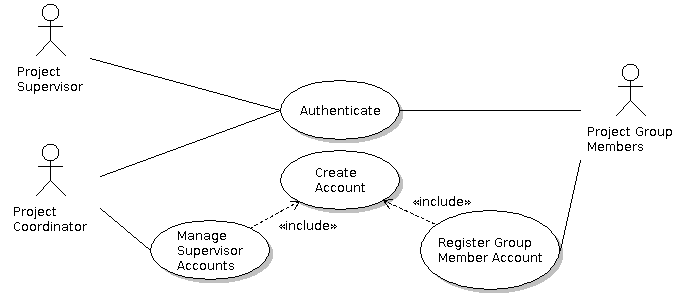
\includegraphics[width=6in]{./img/case-study-fourth-year-system/setup-and-provisioning}
\caption{Use case diagram for the account management functionality of the fourth-year project management system.}
\label{fig:case-4ys-use-case-account-management}
\end{figure}

\begin{figure}[!ht]
\centering 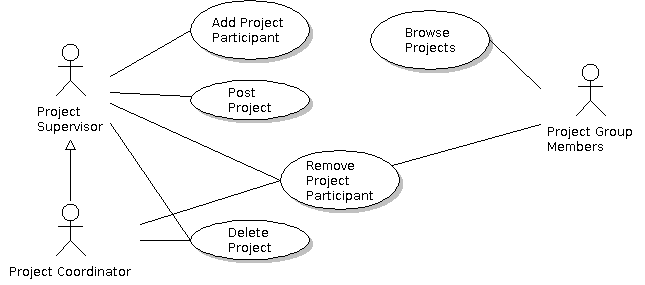
\includegraphics[width=6in]{./img/case-study-fourth-year-system/project-selection}
\caption{Use case diagram for the project selection functionality of the fourth-year project management system.}
\label{fig:case-4ys-use-case-project-selection}
\end{figure}

\begin{figure}[!ht]
\centering 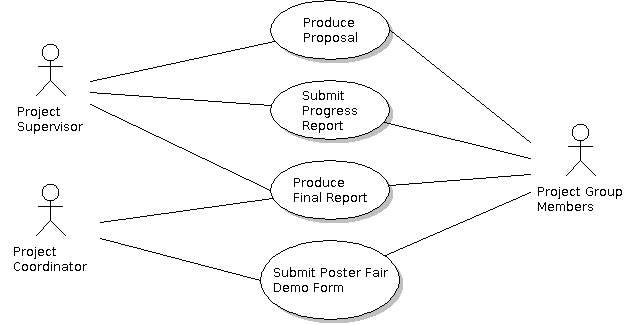
\includegraphics[width=6in]{./img/case-study-fourth-year-system/project-lifecycle}
\caption{Use case diagram for the project execution functionality of the fourth-year project management system. Note that functions related to oral presentations are broken out in Figure \ref{fig:case-4ys-use-case-oral-reports} instead.}
\label{fig:case-4ys-use-case-project-lifecycle}
\end{figure}

\begin{figure}[!ht]
\centering 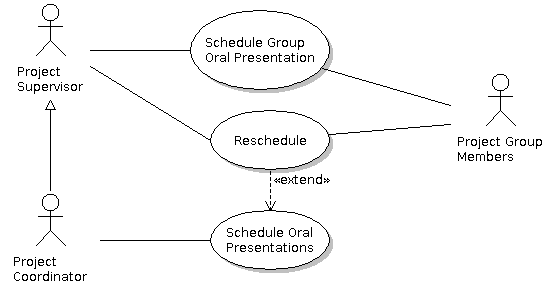
\includegraphics[width=6in]{./img/case-study-fourth-year-system/oral-report-scheduling}
\caption{Use case diagram for the oral presentation functionality of the fourth-year project management system.}
\label{fig:case-4ys-use-case-oral-reports}
\end{figure}

Though all three concerns are important to the system, the most interesting from the point of view of a workflow framework is the project execution phase. This phase accounts for the majority of the lifetime of a fourth-year project, and is also the area in the existing fourth year project management system that could use the most improvement. While account creation and project selection mostly involve basic CRUD (create, read, update, and delete) actions, the execution phase has a well-defined flow:
\begin{enumerate}
\item First, a project proposal must be drafted, submitted, revised, and accepted.
\item After the proposal is accepted, an oral presentation scheduling form must be filled out.
\item Concurrently with scheduling an oral presentation, a progress report must be prepared and submitted.
\item After the progress report is accepted, an oral presentation must be given.
\item After the oral presentation, the group must prepare a presentation for the poster fair. Though this activity has no online deliverables, the group may opt to fill out a poster fair demo request form.
\item While the group is preparing for the poster fair, a final report must also be drafted, submitted, revised, and accepted.
\end{enumerate}
Additionally, each step of the fourth-year project process has associated deadlines.